\section*{Цель работы}

\begin{enumerate}
    \item Получение передаточной характеристики и семейства
    выходных характеристик полевого транзистора;
    \item Расчёт схемы автоматического смещения полевого
    транзистора;
    \item Исследование усилительного каскада по схеме с общим
    истоком.
\end{enumerate}



\section*{Исходные данные}

Все исследования, проводимые в лабораторной работе, выполняются с 
полевым транзистором HAT2164H согласно 16 варианту.
Технические характеристики транзистора:
\begin{itemize}
    \item Ток стока $I_{C}=60\ A$;
    \item Напряжение сток-исток $U_\text{\text{СИ}}=30\ \text{В}$;
    \item Пороговое напряжение затвора $U_\text{пор}=0.8\dots2.3\ \text{В}$;
    \item Рассеиваемая мощность $P=30\ \text{Вт}$.
\end{itemize}


\section*{Снятие передаточной ВАХ полевого транзистора}

Для снятия передаточной ВАХ полевого транзистора в программной среде LTspice 
соберем схему как на рисунке \ref{fig:схема_перед_вах}, после симуляции
получим график зависимости $I_C=f(U_\text{ЗИ})$ (см. Рис. \ref{fig:перед_вах}) при постоянном напряжении 
источника питания равном 10 В.


\begin{figure}[H]
    \centering
    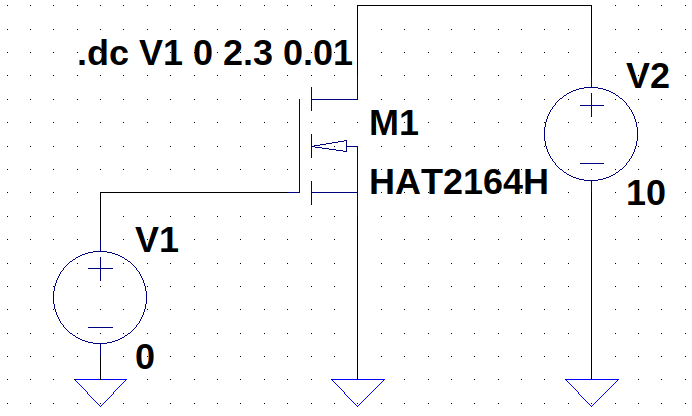
\includegraphics[width=\linewidth]{figs/task_1_scheme.png}
    \caption{Схема для снятия ВАХ полевого транзистора}
    \label{fig:схема_перед_вах}
\end{figure}

\begin{figure}[H]
    \centering
    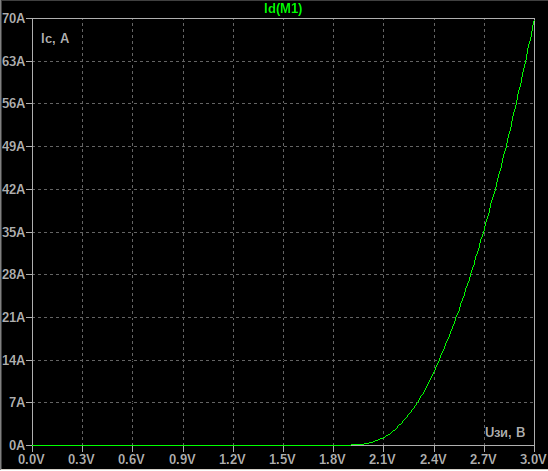
\includegraphics[width=0.8\linewidth]{figs/task_1_перед_хар.png}
    \caption{Передаточная ВАХ полевого транзистора}
    \label{fig:перед_вах}
\end{figure}



\section*{Снятие выходных ВАХ полевого транзистора}

Для получения выходной ВАХ воспользуемся той же схемой как на рисунке \ref{fig:схема_перед_вах},
зависимость $I_C=f(U_\text{СИ})$ при напряжении затвор-исток от 3 до 10 В можно
увидеть на рисунке \ref{fig:выход_вах}.

Крутизна определяется как отношение приращения тока стока $\Delta I_C=36.3\ A$ к изменению 
входного напряжения $\Delta U_\text{ЗИ}=421.6\ \text{мВ}$ при постоянном $U_\text{СИ}$
(см. Рис. \ref{fig:коэффициент_крутизны}):
\begin{equation*}
    S=\frac{\Delta I_C}{\Delta U_\text{ЗИ}}=86.2\ \frac{A}{B}.
\end{equation*}

Выходная проводимость представляет собой
дифференциальную проводимость канала транзистора и
определяется как отношение приращения тока стока $\Delta I_C=24.2\ A$ к
изменению выходного напряжения $\Delta U_\text{СИ}=12.0\ B$ при постоянном $U_\text{ЗИ}$
(см. Рис. \ref{fig:коэффициент_выходной_проводимости}):
\begin{equation*}
    G=\frac{\Delta I_C}{\Delta U_\text{СИ}}=2.0\ \frac{A}{B}.
\end{equation*}

Внутреннее (или выходное) сопротивление полевого
транзистора
\begin{equation*}
    R_i=\frac{\Delta U_\text{СИ}}{\Delta I_C}=0.5\ \text{Ом}.
\end{equation*}


\begin{figure}[H]
    \centering
    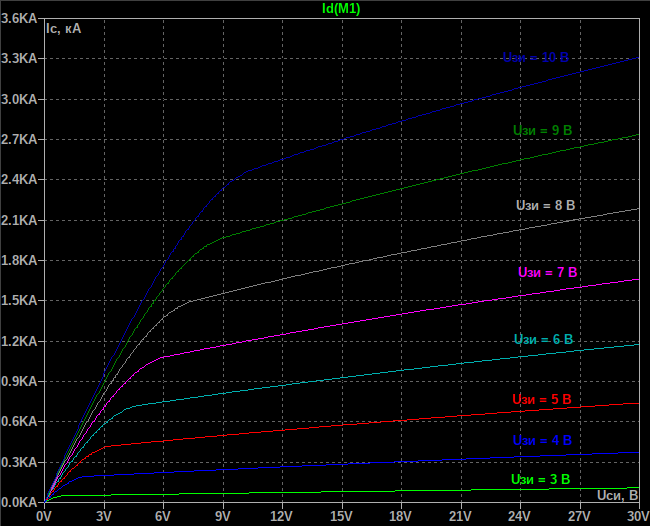
\includegraphics[width=0.8\linewidth]{figs/task_2_выход_вах.png}
    \caption{Выходная ВАХ полевого транзистора}
    \label{fig:выход_вах}
\end{figure}

\begin{figure}[H]
    \centering
    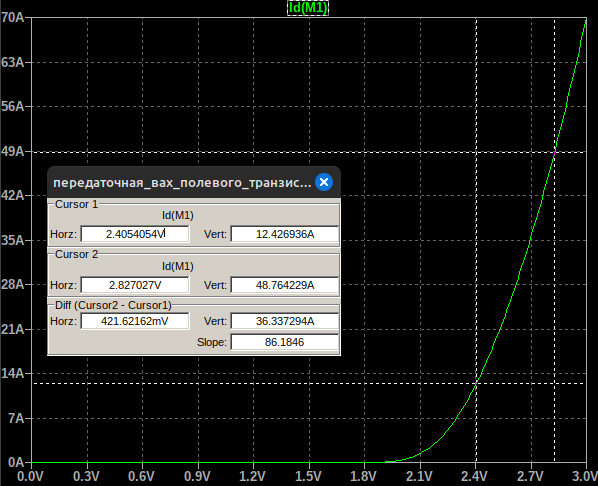
\includegraphics[width=0.8\linewidth]{figs/получение_S.png}
    \caption{Получение коэффициента крутизны}
    \label{fig:коэффициент_крутизны}
\end{figure}

\begin{figure}[H]
    \centering
    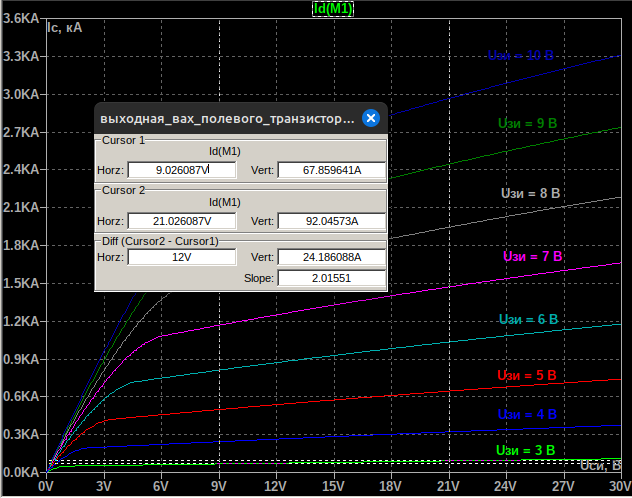
\includegraphics[width=0.8\linewidth]{figs/получение_G.png}
    \caption{Получение коэффициента выходной проводимости}
    \label{fig:коэффициент_выходной_проводимости}
\end{figure}



\section*{Задание рабочей точки усилительного каскада с общим
истоком}

На выходной ВАХ построим линию максимальной мощности (см. Рис. \ref{fig:рабочая_точка}).
На ВАХ в рабочем диапазоне нанесем нагрузочную линию (см. Рис. \ref{fig:рабочая_точка}),
выбрав значение напряжения источника питания $E_\text{К}=12\ B$ и $I_\text{КЗ}=9\ A$:
\begin{equation*}
    U_{\text{СИ}_0}=6.10\ \text{В},\quad I_{\text{С}_0}=4.44\ A,\quad U_{\text{ЗИ}_0}=2.25\ B.
\end{equation*}
Тогда $R_C=1.33\ \text{Ом}$, $R_1=43\ \text{МОм}$, $R_2=10\ \text{МОм}$. Собрем
схему как на рисунке \ref{fig:общий_исток} только без источника напряжения V1 и
конденсатора С1, чтобы проверить рабочую точку. После симуляции получим значения
\begin{equation*}
    U_{\text{СИ}}=6.12\ \text{В},\quad I_{\text{С}}=4.90\ A,\quad U_{\text{ЗИ}}=2.26\ B,
\end{equation*}
как видно значения похожи на рабочую точку, отличается сильнее всего сила тока
стока.

Проведем моделирование схемы \ref{fig:общий_исток} при гармоническом
входном сигнале с амплитудой 0.1 В и частотой 1 кГц. Осциллограммы входных и выходных токов и
напряжений на рисунках \ref{fig:гарм_ток} и \ref{fig:гарм} соответственно.

Рассчитаем коэффициент усиления по напряжению:
\begin{equation*}
    K_U=\frac{U_{\text{ВЫХ}_{max}}}{U_{\text{ВХ}_{max}}}=\frac{2.85\ V}{99.89\ mV}
    \approx 2.85\ .
\end{equation*}
Проведем его частотный анализ (см. Рис. \ref{fig:ачх}). Амплитуда схему не
изменяется до 10 МГц, после чего уже на 100 МГц начинает сильно падать, фаза
смещается постоянно, и чем больше частота тем меньше фаза.

\begin{figure}[H]
    \centering
    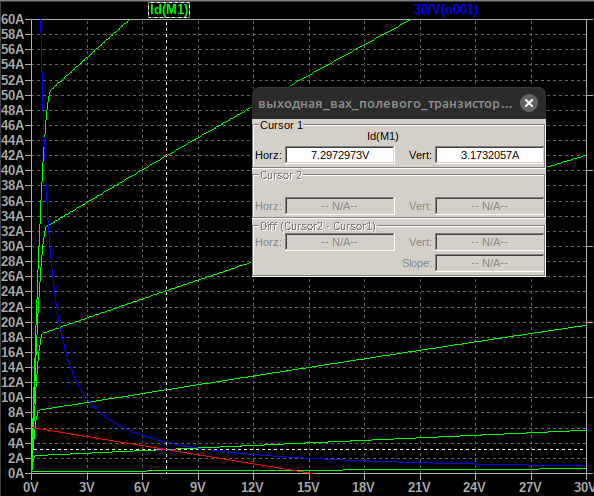
\includegraphics[width=0.8\linewidth]{figs/рабочая точка.png}
    \caption{Рабочая точка усилительного каскада с общим истоком}
    \label{fig:рабочая_точка}
\end{figure}

\begin{figure}[H]
    \centering
    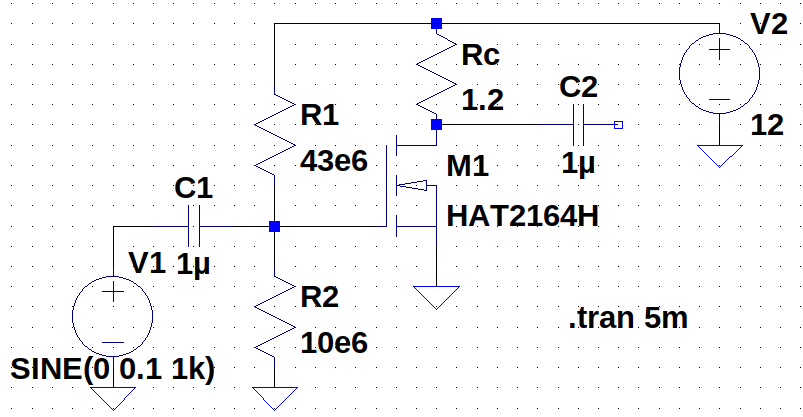
\includegraphics[width=\linewidth]{figs/схема_общий_исток.png}
    \caption{Схема усилительного каскада с общим истоком}
    \label{fig:общий_исток}
\end{figure}

\begin{figure}[H]
    \centering
    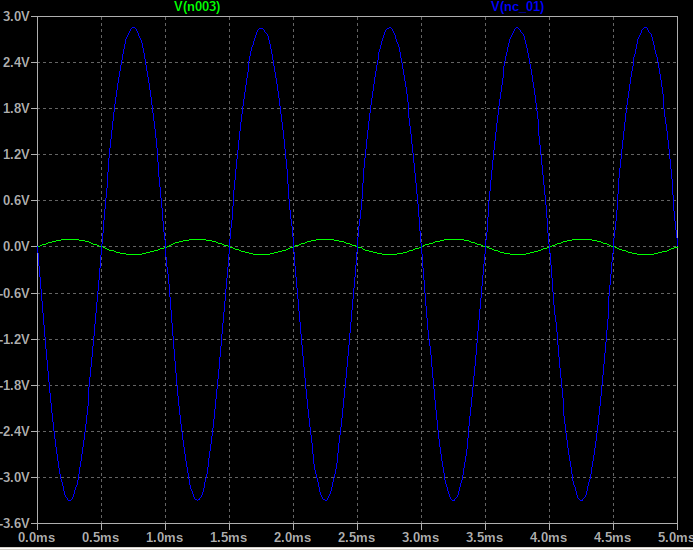
\includegraphics[width=0.8\linewidth]{figs/гарм.png}
    \caption{Осциллограммы входных и выходных напряжений}
    \label{fig:гарм}
\end{figure}

\begin{figure}[H]
    \centering
    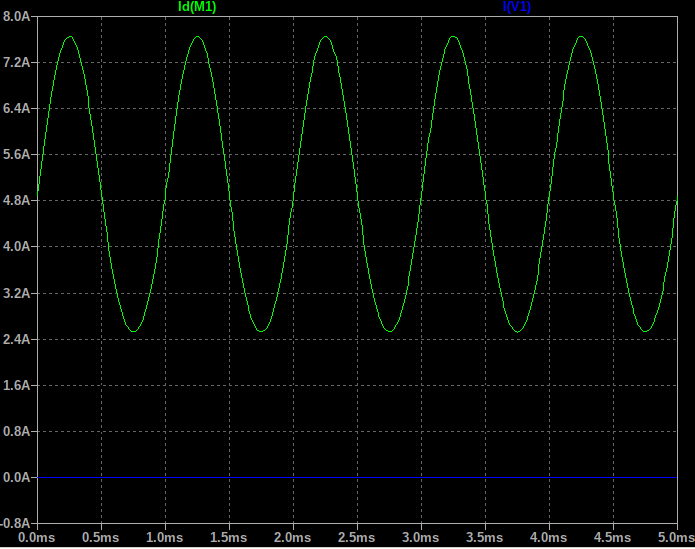
\includegraphics[width=0.8\linewidth]{figs/гарм_ток.png}
    \caption{Осциллограммы входных и выходных токов}
    \label{fig:гарм_ток}
\end{figure}

\begin{figure}[H]
    \centering
    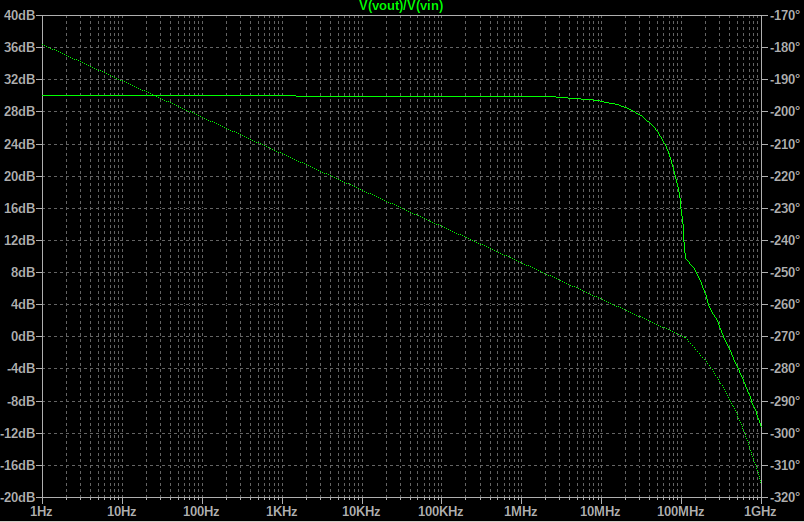
\includegraphics[width=0.8\linewidth]{figs/ачх.png}
    \caption{АЧХ коэффициента усиления по напряжению схемы с общим истоком}
    \label{fig:ачх}
\end{figure}


\section*{Заключение}

В ходе лабораторной исследовали передаточную и выходную ВАХ МОП-транзистора с 
индуцированным каналом: HAT2164H, 
также рассмотрели одно из его применений, а именно транзистор как
усилитель в схеме с общим истоком. Для оценки усиления использовался коэффициент 
усиления напряжения, который составил $2.85$.
